	
	\documentclass[17pt]{extreport}
	\usepackage[utf8x]{inputenc}
	\usepackage[english]{babel}
	\usepackage{url}
	\usepackage{graphicx}
	\usepackage{imakeidx} % for how to use the index see https://www.sharelatex.com/learn/Indices
	\usepackage{hyperref}
	\usepackage[margin=0.6in]{geometry}
	\usepackage{afterpage}
	
	\newcommand\blankpage{%
	    \null
	    \thispagestyle{empty}%
	    \addtocounter{page}{-1}%
	    \newpage}
	
	
	%\title{Trash Magic Action Coloring Book}
	%\author{Trash Robot}
	
	\begin{document}
	
	%\thispagestyle{empty}
	%\mbox{}
	%\maketitle

        \begin{figure}
		\centering
		
\includegraphics[width=6.25in]{imageserver/uploadimages/cover.png}
	\end{figure}
	
        \begin{figure}
		\centering
		
\includegraphics[width=6.25in]{imageserver/uploadimages/trashrobot.png}
	\end{figure}

		
	\begin{figure}
		\centering
		
\includegraphics[width=6.25in]{imageserver/uploadimages/image12.png}
%		\caption{Magic.  Replication in all directions.}
	\end{figure}

	\begin{figure}
		\centering
		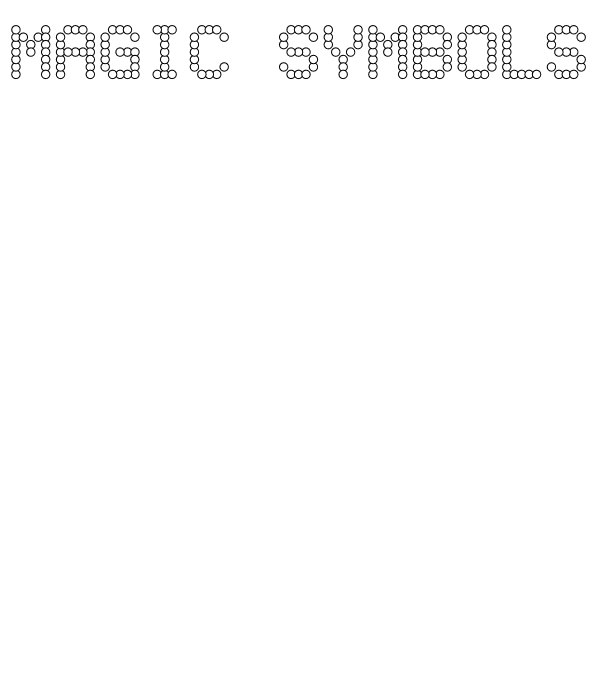
\includegraphics[width=6.25in]{imageserver/uploadimages/magicsymbols.png}
%		\caption{Magical symbology. What are our symbols? What represents who we are and what that means?  What are our most organic symbols, which most freely replicate from person to person?}
	\end{figure}

	
	\begin{figure}
		\centering
		
\includegraphics[width=6.25in]{imageserver/uploadimages/image13.png}
		%\caption{Magic trash.}
	\end{figure}
	
	\begin{figure}
		\centering
		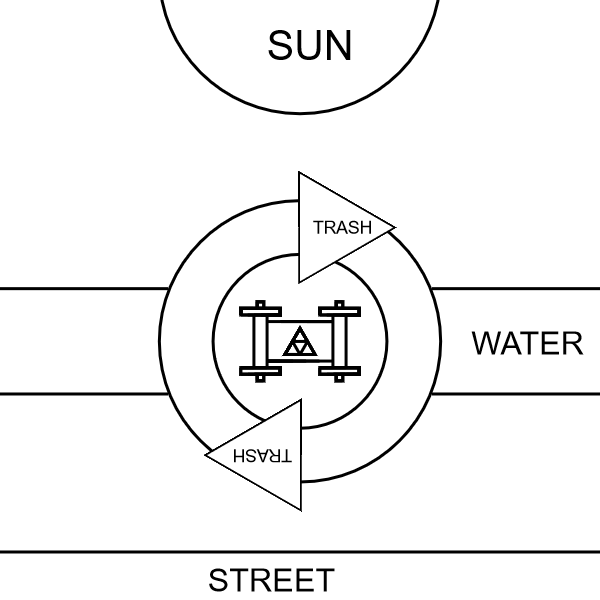
\includegraphics[width=6.25in]{imageserver/uploadimages/image14.png}
%		\caption{Trash magic map.}
	\end{figure}
	
	\begin{figure}
		\centering
		
\includegraphics[width=6.25in]{imageserver/uploadimages/trashgraph.png}
%		\caption{Trash magic graph.}
	\end{figure}
	
	\begin{figure}
		\centering
		
\includegraphics[width=6.25in]{imageserver/uploadimages/trashfactory.png}
		%\caption{Trash Factory. List the things available from the trash factory here.  What are the products, and how can people get them?}
	\end{figure}
	
	\begin{figure}
		\centering
		
\includegraphics[width=6.25in]{imageserver/uploadimages/trashfeed.png}
%		\caption{Trash Feed. Where are we getting trash from? What trash? From whom?  List trash sources, people, places, things.}
	\end{figure}
	
	\begin{figure}
		\centering
		
\includegraphics[width=6.25in]{imageserver/uploadimages/community.png}
%		\caption{Community resources. Our whole purpose is to provide aid to the community. List community resources here.  Who needs what, and how can they get it? Post contact information of both those in need and those willing to help.}
	\end{figure}
	
	
	\begin{figure}
		\centering
		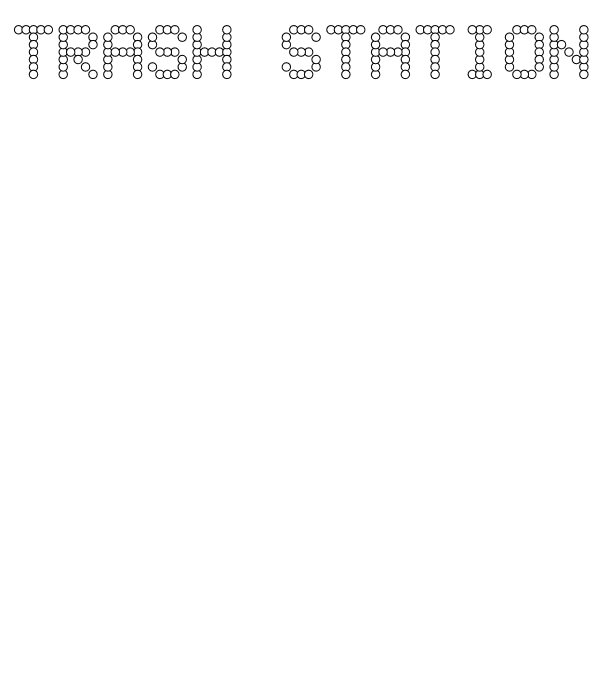
\includegraphics[width=6.25in]{imageserver/uploadimages/trashstation.png}
	%	\caption{Trash Camp. Where are we hanging out?  Details of a spot go here, this can be maker spaces, schools, community centers, parks, or just spaces we can exist.  Draw maps, list places, add links.}
	\end{figure}
	
	
	\begin{figure}
		\centering
		
\includegraphics[width=6.25in]{imageserver/uploadimages/trashacademy.png}
		%\caption{Trash Academy: Teaching. Who is teaching what, and where?  List of what's offered and who teaches it and where they are, contact info of teachers, links to resources to learn.}
	\end{figure}
	
	\begin{figure}
		\centering
		
\includegraphics[width=6.25in]{imageserver/uploadimages/trashlabs.png}
%		\caption{Trash Labs: Research and Development.  Research path.  What do we need to figure out how to build next? What are we working on now?}
	\end{figure}

	\begin{figure}
		\centering
		
\includegraphics[width=6.25in]{imageserver/uploadimages/image16.png}
%		\caption{Scroll.}
	\end{figure}
	
	\begin{figure}
		\centering
		
\includegraphics[width=6.25in]{imageserver/uploadimages/image17.png}
%		\caption{Infinite scrolls.}
	\end{figure}
	
	\begin{figure}
		\centering
		
\includegraphics[width=6.25in]{imageserver/uploadimages/magicbook.png}
%		\caption{This book.  Notes on this book, self-documenting. Where it went, where it goes.}
	\end{figure}
	
	
	 \begin{figure}
		\centering
		
\includegraphics[width=6.25in]{imageserver/uploadimages/streets.png}
	%	\caption[streetmaps]
	%	{Draw maps for the region's streets, one for the major highway corridor, one for local major streets and one for the specific neighborhood.}
	\end{figure}
	
	 \begin{figure}
		\centering
		
\includegraphics[width=6.25in]{imageserver/uploadimages/watershed.png}
	%	\caption[watermaps]
	%	{Draw maps for the region's water, one for the ocean and major shorelines of your watershed, one for major rivers or lakes and one for immediate drainage.}
	\end{figure}
	
	 \begin{figure}
		\centering
		
\includegraphics[width=6.25in]{imageserver/uploadimages/travels.png}
	%	\caption[people]
%		{The path of this book: people.  Put your name, logo, symbols, signs, links, social media, contact as you see fit, then pass the book along to the next person.}
	\end{figure}
	
	
	\begin{figure}
		\centering
		
\includegraphics[width=6.25in]{imageserver/uploadimages/circles6.png}
		%\caption{Circles.}
	\end{figure}

	
	\begin{figure}
		\centering
		
\includegraphics[width=6.25in]{imageserver/uploadimages/image4.png}
	%	\caption{Pentagram.}
	\end{figure}
	
	\begin{figure}
		\centering
		
\includegraphics[width=6.25in]{imageserver/uploadimages/image5.png}
	%	\caption{Hexagon.}
	\end{figure}
	
	\begin{figure}
		\centering
		
\includegraphics[width=6.25in]{imageserver/uploadimages/image6.png}
		%\caption{Elements.}
	\end{figure}
	
	\begin{figure}
		\centering
		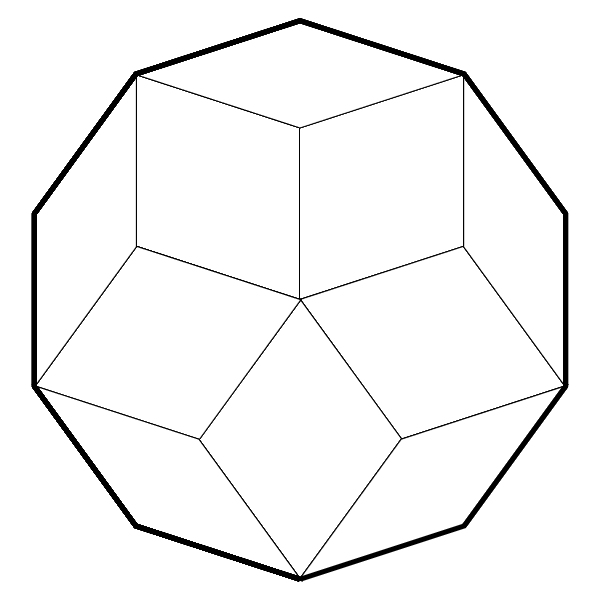
\includegraphics[width=6.25in]{imageserver/uploadimages/image7.png}
		%\caption{Penrose.}
	\end{figure}
	
	\begin{figure}
		\centering
		
\includegraphics[width=6.25in]{imageserver/uploadimages/image18.png}
		\caption{Golden Spiral.}
	\end{figure}
	
	\begin{figure}
		\centering
		
\includegraphics[width=6.25in]{imageserver/uploadimages/qubert.png}
	\end{figure}


	\begin{figure}
		\centering
		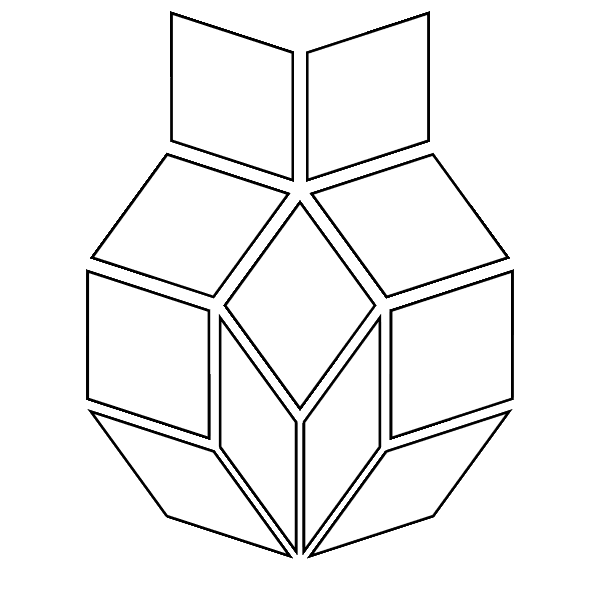
\includegraphics[width=6.25in]{imageserver/uploadimages/pi.png}
%		\caption{Raspberry pi pattern for stitching felt onto bags.}
	\end{figure}
	
	\begin{figure}
		\centering
		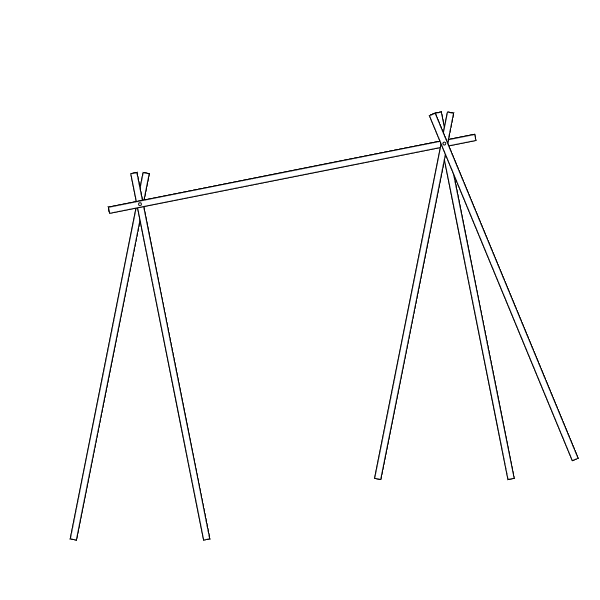
\includegraphics[width=6.25in]{imageserver/uploadimages/image9.png}
%		\caption{Skeletron.}
	\end{figure}
	
	\begin{figure}
		\centering
		
\includegraphics[width=6.25in]{imageserver/uploadimages/image10.png}
%		\caption{S Hook.}
	\end{figure}
	
	\begin{figure}
		\centering
		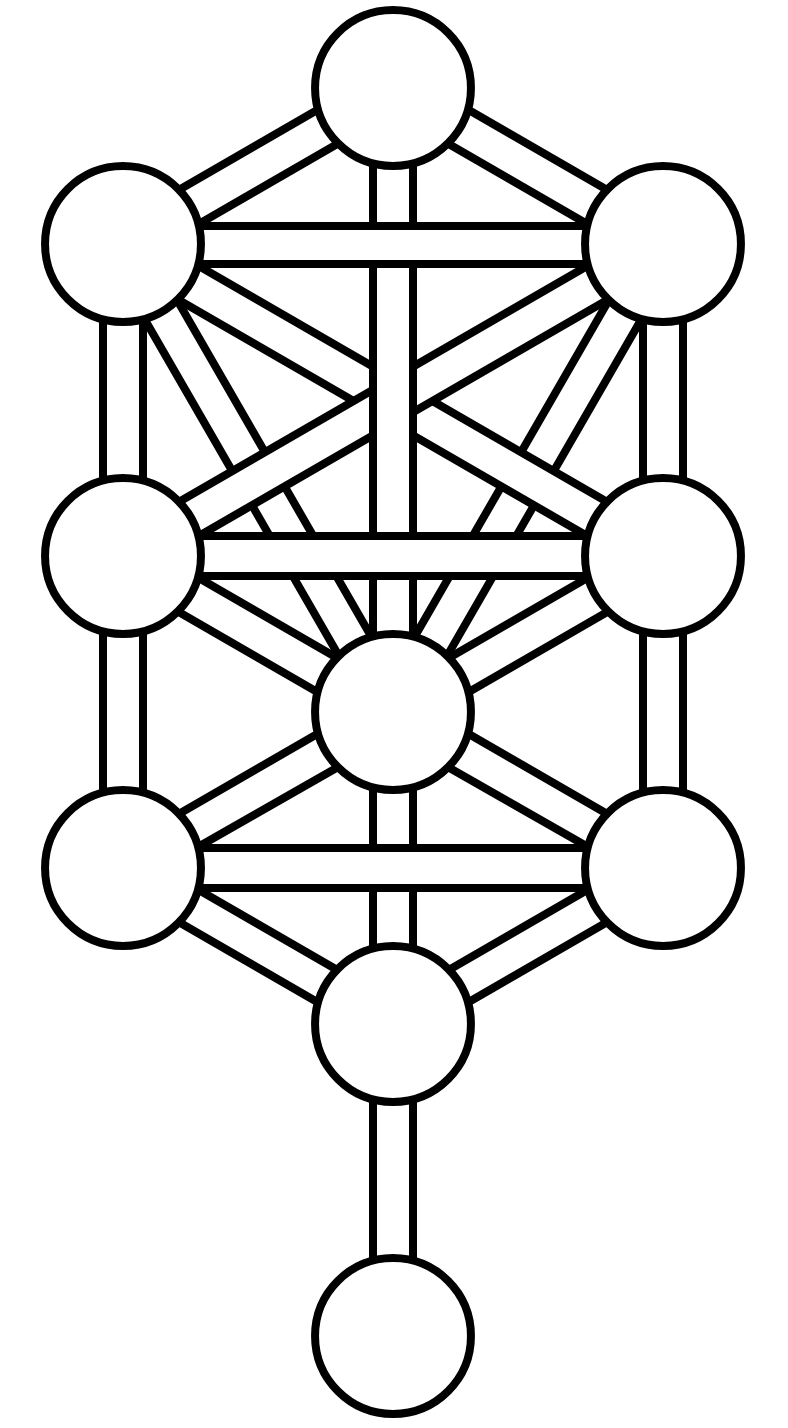
\includegraphics[width=3in]{imageserver/uploadimages/image1.png}
%		\caption{Tree of life.}
	\end{figure}
	
	
	
	
	\end{document}